Using the original data set (“PassengersNormal”) as the basis of comparison, several conclusions could be drawn regarding the models' efficiency or inefficiency and the reasons for it. The time differences for each specific measurement mentioned in chapter 4 were summarized in the following table:
\begin{table}[H]
  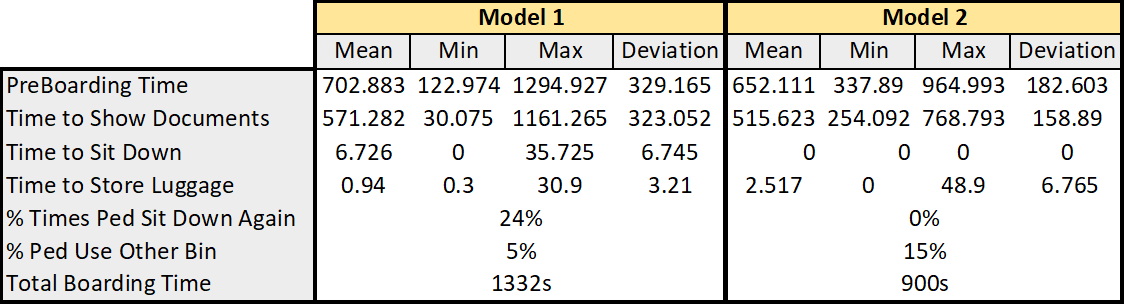
\includegraphics[width=1.0\textwidth]{tables/statistics.png}
  \caption{Time Statistics - Model 1 \& 2}
  \label{tbl:statistics}
\end{table}
Starting with the pre-boarding time, in the first model most passengers have to wait for groups with higher priority to enter the plane first, and even though the second model's system establishes an even more specific entrance sequence, the average time passengers spend waiting to show their documentations from the moment they get to the waiting area is 702.883 seconds for Model 1 and 652.111 seconds for Model 2. The same happens when just considering how long it takes for passengers to get to the staff verifying the documentation. This can probably be explained by both models checking if everyone has arrived at the waiting area before enabling passengers to form a queue. It should be noticed, however, that the lowest waiting time values were obtained in Model 1 as, because of the data set file, the first passengers to arrive are people with special needs, who can immediately start boarding.

\indent\newline
Moving onto the time passengers take to sit down, as expected, there is absolutely no interference in Model 2 in the sense that no passenger has to get up from their seat in order to let another passenger sit down in the same sitting block. On the other hand, Model 1 does not avoid nor minimize this concern. At the most extreme case, a passenger already standing in front of their sitting block still had to wait 35.725 seconds to sit down. Consequently, whereas in Model 1 24\% of the passengers kept leaving their seat and sitting down again, in Model 2 this percentage is reduced to 0.
Interestingly enough, Model 1 did overcome Model 2 in one aspect: the time spent storing luggage. Neither model was prepared to optimize the search for other bins when the one above the passenger's seat is full and so in both models passengers move along the aisle trying to store their bags. But neither one is clearly superior either. To put it simply, the particular data set associating the amount of luggage per passenger turned out more favorable for Model 1 than for Model 2, resulting in an average searching time of 0.94 seconds for the first and of 2.51 seconds for the latter. This was also reflected in the percentage of passengers looking for alternative bins: 15\% for Model 2 and only 5\% for Model 1. So not only did passengers take more time to store their luggage but also more passengers had trouble finding room left for their belongings.
\indent\newline
This said, overall Model 2 was much more efficient, resulting in a total boarding time of 900 seconds whereas Model 1 took longer to finish: 1332 seconds.
